
\documentclass[preprint]{sigplanconf}

% The following \documentclass options may be useful:

% preprint      Remove this option only once the paper is in final form.
% 10pt          To set in 10-point type instead of 9-point.
% 11pt          To set in 11-point type instead of 9-point.
% authoryear    To obtain author/year citation style instead of numeric.

\usepackage{amsmath}
\usepackage{amssymb}
\usepackage{amsthm}
\usepackage{amsfonts}
\usepackage{pifont}
\usepackage{listings}
\usepackage{graphicx}
\usepackage{xspace}
\usepackage{pgf}
\usepackage[noend]{algpseudocode}
\usepackage{algorithm}
\usepackage{multicol}
\usepackage{appendix}
\usepackage{caption}
\DeclareCaptionType{copyrightbox}
\usepackage{subfig}
\usepackage{multirow}
\usepackage{tikz}
\usetikzlibrary{arrows, automata, shapes}

\newtheorem{theorem}{Theorem}
\newtheorem{lemma}[theorem]{Lemma}
\newtheorem{corollary}[theorem]{Corollary}
\newtheorem{conjecture}[theorem]{Conjecture}

\theoremstyle{definition}
\newtheorem{definition}[theorem]{Definition}

\newcommand{\xmark}{\ding{55}}
\newcommand{\todo}[1]{{\bf TODO:} #1}

\lstset{language=c++}



\begin{document}

%\special{papersize=8.5in,11in}
\setlength{\pdfpageheight}{\paperheight}
\setlength{\pdfpagewidth}{\paperwidth}

\conferenceinfo{POPL '14}{Month d--d, 20yy, City, ST, Country} 
\copyrightyear{2014} 

% Uncomment one of the following two, if you are not going for the 
% traditional copyright transfer agreement.

%\exclusivelicense                % ACM gets exclusive license to publish, 
                                  % you retain copyright

%\permissiontopublish             % ACM gets nonexclusive license to publish
                                  % (paid open-access papers, 
                                  % short abstracts)

\title{Synthesising Complex Termination Arguments}

\authorinfo{Cristina David\and Daniel Kroening\and Matt Lewis}
           {Oxford University}
           {firstname.lastname@cs.ox.ac.uk}

\maketitle

\begin{abstract}
Proving program termination is typically done by finding a well-founded \emph{ranking function}
for the program states.
Existing termination provers typically find ranking functions
using either linear algebra or templates.  As such they are often restricted to
finding linear ranking functions over mathematical integers.  This class
of ranking functions is not large enough to prove termination for all terminating
programs, and furthermore a termination argument for a program operating on mathematical integers
does not always lead to a termination argument for the same program operating on
fixed-width machine integers.

We present a reduction from program \emph{termination} to program \emph{synthesis}.
This reduction allows us to generate nonlinear, lexicographic ranking functions that
are correct for fixed-width machine arithmetic and floating-point arithmetic.
We use this reduction to build a semi-decision procedure for the termination
of fixed-width and floating-point arithmetic programs.
\end{abstract}

%\category{CR-number}{subcategory}{third-level}


\keywords
Termination, Program Synthesis, Lexicographic Ranking Functions, Bitvector Ranking Functions,
Floating Point Ranking Functions.

\section{Introduction}

Proving program termination is typically done by finding a well-founded \emph{ranking function}
for the program states. When doing so, the majority of the existing termination provers diverge 
in one important aspect from the execution
of a program on a computer:
bit-vectors and floats 
are treated as mathematical integers and reals, respectively \cite{}.
This approximation gives rise to 
{\em unsound} and {\em incomplete} analyses, which is rather surprising given that bit-vectors and floats are ubiquitous in computer systems. 



For the case of bit-vectors (machine-level integers), their abstraction  to mathematical integers 
ignores the wrap-around behaviour caused by under/over-flows in bit-vector arithmetic, resulting in %, it gives rise to 
%{\em unsound} and {\em incomplete} analyses, which is rather surprising given that bit-vectors are ubiquitous in computer systems. 
incomparable behaviours with respect to termination:
%The differences between the semantics of unbounded mathematical integers and that of machine integers result in 
\begin{itemize}
\item Programs that terminate for integers may \emph{not} terminate for bit-vectors. For illustration, consider the following loop:
\begin{lstlisting}[language=C]
while (x > 0) x -= 2;
\end{lstlisting}
The loop always terminates for unbounded integers as the value of \texttt{x} does eventually become negative, 
whereas, with bit-vector arithmetic, \texttt{x} under-flows before becoming negative and goes back to being positive causing the loop to never terminate.
According to the C11 standard for the C programming language, a signed under- or over-flow yields undefined behaviour.
However, compilers generally treat signed under- and over-flows using the
wrap-around behaviour (see Section~\ref{}). 
\item Similarly, programs that terminate for bit-vectors may \emph{not} terminate for integers. One such situation is illustrated next:  
 \begin{lstlisting}[language=C]
 while(x > 0) x++;
 \end{lstlisting}
This loop is  terminating for bit-vectors since \texttt{x}
will eventually over-flow and become negative. Conversely, the same program is non-terminating using integer
arithmetic since the loop condition stays always true for any initial \texttt{x} at least 1.
\end{itemize}

A scenario similar to the one for bit-vectors happens when floats are abstracted to unbounded reals by termination provers \cite{}.
Consequently, these provers ignore potential rounding errors, under- and over-flows, which are precisely what makes  reasoning about floating point inherently difficult.
This approximation may lead to erroneous diagnosis of a program's terminating behaviour as illustrated next:
\begin{itemize}
\item This loop does not terminate for reals, but does for floats.
\begin{lstlisting}
while (x > 0.0) x *= 0.5;
\end{lstlisting}

\item The following loop terminates for reals, but does not for floats.
\begin{lstlisting}
while (x > 0.0) x -= 1.0;
\end{lstlisting}
\end{itemize}   
\todo{explain the reasons for non-termination with figures.}


Another limitation of the state of the art in the computation of ranking functions is the fact that  most techniques assume \emph{restrictive transition relations} and are only able to compute
\emph{linear ranking functions} \cite{}. To better understand this restriction, we computed the probability of a random terminating program having a linear ranking
function (see Section ?). This probability proved to be very low, indicating that the linearity assumption for the ranking functions is indeed prohibitive.

Because most state-of-the-art termination procedures use disjunctive well foundedness arguments, they require the use of
complex safety provers that are able to reason about unbounded unfoldings of a transition relation.  In contrast to this,
we are able to build monolithic termination arguments that only need ``local'' reasoning -- our ranking functions
can be proved sufficient by considering just a single unfolding of a loop.

Many loops do not terminate for all starting states, but are contained in programs that guarantee the loop will
terminate.  Traditional termination provers have difficulty reasoning about such conditionally-terminating loops.
We are able to handle such loops by computing \emph{termination invariants}.  This mechanism also allows us to
prove that programs with multiple loops terminate, even if the termination of some loop depends on the states
reachable after leaving a previous loop.

We propose a general framework that does not assume the existence of linear ranking functions and can uniformly compute
(lexicographic) linear and non-linear ones, 
for programs with both bit-vectors and floats. Our technique can handle programs with non-linear operations, e.g. logical and.
For this purpose, we rephrase the termination problem as a second-order satisfaction problem
(indeed, a program synthesis problem). 
As a direct consequence, our technique is semantic in nature and does not
dependent on the size of the analysed program or its number of variables. 
However, its efficiency does depend on the Kolmogorov
 complexity of the computed ranking functions. We show that the probability of
a ranking function to have a low Kolmogorov complexity is higher than the probability to be linear (see Section~?).

By phrasing the termination problem as a single rank function synthesis problem, we observe that
we can make the termination problem as hard as finding ranking functions, rather than as hard as
solving a difficult ``double reachability'' problem (cf. Terminator).

\begin{figure}
 \begin{tabular}{|ll||c|c|}
 \hline
  & & \multicolumn{2}{c|}{Program} \\
  & & Linear & Non-Linear \\
  \hline
  \hline
  \multirow{2}{*}{Ranking Functions} & Linear & \checkmark \xmark & \checkmark \\
   & Non-Linear & \checkmark & \checkmark \\
   \hline
 \end{tabular}

 \caption{Legend: \xmark = state-of-the art can handle, \checkmark = we can handle\label{fig:handletable}}
\end{figure}


%We empirically observe that most programs have
%ranking functions with low Kolmogorov complexity (see Section ?). 

%Church was BIG into program synthesis~\cite{church-synth}, so you know it's good stuff.
%Something, something, Curry-Howard Isomorphism, something, something, programs-as-proofs.

The main contributions of our paper are highlighted below:
\begin{itemize}
\item We designed a technique for computing ranking functions that correctly accounts for the wrap-around behavior caused by under- and overflows in bit-vector and floating point arithmetic. To the best of our knowledge, this is the first approach able to compute ranking functions for programs handling floats. Our technique is not restricted to finding linear ranking functions, but can also compute (lexicographic) non-linear  ones. We justified the need for such a non restrictive procedure by computing the probability ... .
\item  We rephrased the termination problem as a second-order satisfaction problem and made 
use of results in genetic programming to efficiently solve it. We have also investigated the effects of genetic operators on the search space for ranking functions and computed theoretical 
bounds on the convergence time ...
\item We present a formulation that allows us to prove termination without using a fancy safety prover (because
we don't do a DWF proof).  In particular,
we only need a bounded model checker that performs a single unwinding of a loop.
\item Our technique is able to uniformly handle conditionally-terminating loops, as well as programs with
multiple loops.
\item We implemented our technique and tried it on a selection of programs handling both bit-vectors and floats.
\end{itemize}

%completeness without disj well-foundedness
%. only non-strict inequalities can be transformed using Farkas’ Lemma


This paper is organised as follows:

\section{Related Work}
\subsection{Termination analysis}
The existing work on termination is primarily divided into structural (syntactic) vs. semantic approaches.  
For example, terminationg of term rewriting systems is largely structural, whereas DWF analysis (cf. Terminator) is more semantic. While it deals
with transition relations, it also uses some amount of syntax in that it identifies loops \& looping paths.

A program is lasso-shaped if it is composed by a stem followed by a single loop without branching, i.e. there is only one path. 
Consequently, the termination argument can be very simple. There are numerous techniques specialised in
proving termination of lasso-shaped programs efficiently \cite{DBLP:conf/popl/Ben-AmramG13,DBLP:conf/cav/BradleyMS05,DBLP:conf/atva/HeizmannHLP13,DBLP:conf/vmcai/P04}. 

Cook et al. are closer to a semantic approach by viewing the termination proving task as a binary reachability analysis \cite{DBLP:conf/pldi/CookPR06}.
%Terminator incrementally constructs the union of ranking relations.
%Given that the this union is not well-founded (it is only disjunctively well-founded), 
%Terminator must prove that the binary reachability relation of the program (the transitive closure of the transition relation restricted to reachable states) 
%is contained in the union of ranking relations.
%Thus, this approach requires an evolved binary reachability, and, implicitly, the assistance of a safety prover.
In particular, their technique incrementally constructs the union of ranking relations.
Given that the this union is not well-founded (it is only disjunctively well-founded),
they must show that, for every sequence, one of the ranking functions decreases
between the pre- and post-state. %In other words: it 
%must find all pairs of states reachable from the program's initial state 
%such that one is reachable from the other and it must show 
%that the value of one of the ranking functions decreases from s1 to s2. 
Consequently, most of the analysis time is spent in reachability analysis that is to check if the current
transition invariant reached a fixed point.

As we want to avoid the requirements of a binary reachability analysis, our termination argument is not a set
of ranking functions, but a single ranking function, which we prove is enough for proving the termination of any termination program. 
With a single ranking function we only need to show that the rank decreases from the
pre- to post-state after executing each single transition step.
The checking process is therefore easy. For the construction of the ranking function, we 
formulate the problem as a second order satisfaction formula and we solve it via program synthesis.

Lee et al. make use of transition predicate abstraction, algorithmic learning, and decision procedures to compute transition
invariants as proofs for the termination of linear programs \cite{DBLP:conf/cav/LeeWY12}.

There is very limited work on generating ranking functions for relations over machine integers.
Cook et al. present a method based on a reduction to Presburger
arithmetic, and a template-matching approach for predefined classes of
ranking functions based on reduction to SAT- and QBF-solving \cite{DBLP:conf/tacas/CookKRW10}.

Leike and Heizmann present a new method for the constraint-based synthesis
of termination arguments for linear loop programs based on
linear ranking templates \cite{DBLP:conf/tacas/LeikeH14}.

Learning: \cite{DBLP:journals/corr/HeizmannHP14}

Polynomial programs: \cite{DBLP:conf/vmcai/BradleyMS05}

%-- Usually the termination argument for the program LOOPS
%on Figure 1 is based on a lexicographic combination
%of well-founded orderings.


%-- the union T of ranking relations, however, is in general not well-founded
%(it is only disjunctively well-founded in the terminology of [23]). This is
%why it would not be sufficient to show the inclusion R \subseteq  T, and why we must in stead prove R_I^+ \subseteq T.

\subsection{Synthesis}

%% ---
%% constructs and checks the termination argument

%% T ERMINATOR’s most distinguishing aspect, with respect to pre-
%% vious methods and tools for proving program termination, is how it
%% shifts the balance between the two tasks of constructing and respec-
%% tively checking the termination argument. The classical method is
%% to construct an expression defining the rank of a state and then to
%% check that its value decreases in every transition from a reachable
%% state to a next one. The construction of the ranking function is the
%% hard part and forms a task that needs to be applied to the whole
%% program. The checking part is relatively easy. In our method, the
%% task of constructing ranking functions is the relatively easy part;
%% they are constructed on demand based on the examination of only
%% a few selected paths through the program.

%% Previously, it was not known whether binary reachability analysis could be made
%% practical. The challenge raised by our approach was to show that
%% this is indeed the case.

%% ----------
%% Efficient synthesis of ranking functions for machine-level bit-vectors, how-
%% ever, has remained an open problem.
%% ---------

\section{Motivational Examples} 
We next discus a few examples that illustrate the difficulties in termination checking for low-level code. In particular, they denote situations that arise 
frequently in low-level code and are not handled by existing techniques. 

%We now present a few examples that justify 

\subsection{A non-linear program with a linear ranking function.}
The first example we consider is a program with non-linear operations: 
\begin{lstlisting}
while (x > 0)
 x = (x - 1) & x;
\end{lstlisting}

In order to find a ranking function for this example, it is necessary to take into account
the semantics of the bit-wise AND operator, which is not easily done when working with mathematical integers \cite{}.
Our technique finds that a possible ranking function is the linear function
$R(x) = x$, whose value decreases with
every iteration, but it can not decrease indefinitely as it is bounded from below.

\subsection{A linear program with a non-linear ranking function.}
\begin{lstlisting}
while (x != 0)
 x = -x / 2;
\end{lstlisting}

\subsection{Differences in the termination behaviour for reals and floats.}
\begin{lstlisting}
while (x > 0.0) x -= 1.0;
\end{lstlisting}

\begin{lstlisting}
while (x > 0.0) x *= 0.5;
\end{lstlisting}

\subsection{A linear program with lexicografic non-linear function.}
\begin{lstlisting}
while ( q >= 0 ) {
  q = q - y;
  y = y + 1;
}
\end{lstlisting}

Every execution of the above program can be partitioned into two phases: in the first phase $y$ increases
until it is positive (in this phase $q$ may increase), whereas in the second $q$ decreases until the loop condition is violated. 
%Depending on the initial values of y and q, either phase might be skipped
%altogether.
\cite{DBLP:conf/tacas/LeikeH14} proposes using a linear ranking template in order to obtain a ranking function that proceeds
through a fixed number of phases in the program execution. Each phase is
ranked by an affine-linear function, and ends when this function becomes non-positive.


Lexicographic non-linear ranking functions consist of lexicographically ordered components
of non-linear functions. As with linear lexicographic ranking functions, a state is mapped to a tuple of values such that the
loop transition leads to a decrease with respect to the lexicographic
ordering for this tuple. Therefore no function may increase unless a function of
a lower index decreases. Additionally, at every step, there must be at least one
function that decreases.


\subsection{Lexicographic ranking function with strict inequalities.}
Approaches based on Farkas’ Lemma can only handle non-strict inequalities \cite{DBLP:conf/cav/BradleyMS05,DBLP:conf/vmcai/P04}.
[2,5,6,7,14,20,24,25

\section{Preliminaries}
\subsection{Termination and Ranking Functions}
A transition system with state space $X$ and transition relation $T \subseteq X \times X$
is said to be \emph{unconditionally terminating} if there is no infinite sequence
$x_1, x_2, \ldots$ with $\forall i . T(x_i, x_{i+1})$.  We can prove that $T$ is
unconditionally terminating by finding an injective function $R: X \to Y$ where
$Y$ is well-founded and $R$ is monotonically decreasing with respect $T$.  That is
to say:
$$\forall x, x' . T(x, x') \Rightarrow R(x) < R(x')$$

A special case of a ranking function is a \emph{linear ranking function}.  This
class of functions is exactly what you'd expect: a linear function that satisfies
the criteria for a ranking function.  We recall that a linear function $f: X \to Y$,
with $\dim(X) = n$ and $\dim(Y) = m$
is one that can be expressed as an $n \times m$ matrix $M$:
$$f(\vec{x}) = M\vec{x}$$

In the case that $\dim(Y) = 1$, this reduces to an inner product:
$$f(\vec{x}) = \vec{\lambda} \cdotp \vec{x} + c$$

If $Y = Z^m$, we say that the ranking function is \emph{lexicographic},
and require that the total order imposed on $Y$ is the lexicographic ordering
induced on tuples of $Z$'s.  We note that some termination arguments
require lexicographic ranking functions, or equivalently, ranking functions
whose co-domain is the ordinals, rather than just $\mathbb{N}$.

\subsection{Disjunctive Well-Foundedness}
Terminator uses disjunctive well foundedness arguments, which can be found
piece by piece, but require reasoning about the transitive closure of a transition
relation.  Because we build a monolithic well foundedness argument, we
do not need to reason about the full transitive closure, and can instead do our
reasoning over a single step of the transition relation.  This means that we
can get away with very simple model checking methods, rather than requiring
a full-blown safety prover.

\subsection{Machine Arithmetic and Bitvectors}
Computers tend to have fixed width integers.  For a machine with $k$-bit words,
all arithmetic is done modulo $2^k$.  This means that a program's termination
behaviour can depend strongly on whether it is interpreted as operating over
mathematical integers, or over fixed-width machine words.  We can however
observe that if no arithmetic operation \emph{overflows} (i.e. does not result
in a value greater than $2^k$), fixed-width and integer arithmetic coincide.

\section{Combinatorics of Finite Termination}
In this section, we fix a model of computation, describe its semantics and
define the syntax of a language we will work over.

\subsection{Syntax and Semantics}

\begin{itemize}
 \item Our transition relation is $T(x, x') \subseteq X \times X$.
 \item Our loop condition is $L(x) \subseteq X$.
 \item Our ranking function is $R(x) : X \to Y$.
 \item Our state space has size $\| X \| = M = 2^k$.
 \item Our ranking co-domain has size $\| Y \| = N = 2^j$.
 \item The number of looping states is $\| L \| = l$.
 \item Our transition relation is deterministic and parititioned into chains of length $c_i$, with $l = \sum c_i$.
\end{itemize}

\subsection{Counting Programs}
\begin{itemize}
 \item There are a TON of programs (way more than you'd expect).
 \item There are a TON of terminating programs, and for our model of computation we can count
  how many (the Chaitin constant).
 \item There are a TON of ranking functions (way more than you'd expect, but not many as a
  fraction of programs).
 \item There are not many linear functions.
 \item Most terminating programs don't admit linear ranking functions.
 \item The Curry-Howard isomorphism
 \item Kolmogorov complexity is relevant for understanding termination proofs.
\end{itemize}


\begin{theorem}
 A random function $f : X \to Y$ is a ranking function for $(T, L)$ with probability

 $$N^{-l} \times \prod {{N-1} \choose c_i}$$
\end{theorem}

\begin{proof}
 Combinatorics.
\end{proof}


\begin{corollary}
 This number is really small (e.g. $10^{-193}$ for a 64-bit program with 1 variable and 10 looping states.
 Randomly sampling functions \& hoping they're ranking functions is not going to work.
\end{corollary}


\begin{conjecture}
 The probability that a random program $(T, L)$ is terminating (the Chaitin constant)
 is $0.7$.
\end{conjecture}

\begin{conjecture}
 The probability that a random program $(T, L)$ admits a linear ranking function is
 $0.1$.
\end{conjecture}

\begin{conjecture}
 The probability that a random, terminating program $(T, L)$ admits a linear ranking function
 is $0.2$.
\end{conjecture}


\begin{corollary}
 Most terminating programs do not have linear ranking functions.
\end{corollary}


\section{Termination as Second-Order Satisfaction}
We can specify the existence of a ranking function, and therefore the termination
of a program, using a second order formula:

\begin{figure*}
\begin{definition}[Second-order Termination Formula]
\begin{align*}
 \exists R . \forall x, x' . & R(x) > 0 ~ \wedge \\
                             & T(x, x') \rightarrow R(x) > R(x')
\end{align*}
\end{definition}

\begin{definition}[Conditional Termination Formula]
 \begin{align*}
  \exists R, I . \forall x, x' . & P(x) \rightarrow I(x) ~ \wedge \\
                                 & c(x) \wedge I(x) \wedge T(x, x') \rightarrow I(x') \wedge R(x) > 0 \wedge R(x) > R(x')
 \end{align*}
\end{definition}

\begin{definition}[Multiple Loops Termination Formula]
 \begin{align*}
  \exists R, I_1, I_2 . \forall x, x' . & P(x) \rightarrow I_1(x) ~ \wedge \\
                                        & I_1(x) \wedge L_1(x, x') \rightarrow I_1(x') ~ \wedge \\
                                        & I_1(x) \wedge \lnot c_1(x) \rightarrow I_2(x) ~ \wedge \\
                                        & c(x) \wedge I_2(x) \wedge L_2(x, x') \rightarrow I_2(x') \wedge R(x) > 0 \wedge R(x) > R(x')
 \end{align*}
\end{definition}
\end{figure*}

Our method for ranking function synthesis can be stated as follows:
discuss what spec is used (non-lexicographic vs lexicographic) + the completeness claims.
Any termination guarantees?  

\section{Second-Order Satisfaction as Program Synthesis}
The program synthesis problem can be described as finding a satisfying assigment to the
synthesis formula:

\begin{definition}[Synthesis Formula]
 The synthesis formula for a specification $\sigma: X \to Y$ is:
 
 $$\exists P \cdotp \forall x \cdotp \sigma(x, P(x))$$
 \end{definition}

Since this formula involves quantification over functions $X \to Y$,
this is a second-order formula -- indeed, if $X = Y = \mathbb{N}$,
the formula describes a set at level $\Sigma_1^1$ of the analytical
hierarchy.  As such, determining the satisfiability of the synthesis
formula over a given logic is strictly harder than solving the
halting problem over the same logic.

\subsection{Generalised Synthesis}
Sometimes we want to synthesise several programs at once, as well as some
ground terms $\vec{x}$.  Also, we might want a more complex specification
than just a relation over $X$ and $Y$.

\begin{definition}[Generalised Synthesis Formula]
 $$\exists P, \vec{x} \cdotp \forall \vec{y} \cdotp \sigma(x, P, y) $$
\end{definition}

\subsection{Reducing Termination to Synthesis}
For a transition system $T$, we can build a specification $\sigma$ to find a conditional ranking function for
$T$ with initial states I:

\begin{eqnarray}
 \sigma(V: X \to \mathbb{B}, R: X \to \mathbb{N}, x, x') = & I(x) \rightarrow V(x) \wedge \\
 & V(x) \wedge T(x, x') \rightarrow V(x') \wedge R(x) < R(x') 
\end{eqnarray}

Here we have synthesised a ranking function $R$ into $\mathbb{N}$ (which is well-founded),
as well as an inductive invariant $V$ that guarantees termination of $T$.

To synthesise an n-place lexicographic ranking function, we just ask for a ranking function
$R: X \to \mathbb{N}^n$.

We recall the definition of the Kolmogorov-complexity of a function $f$:

\begin{definition}[Kolmogorov complexity]
 The Kolmogorov complexity $K(f)$ is the length of the shortest program that
 computes $f$.
\end{definition}

We are primarily interested in studying low-Kolmogorov-complexity (LKC)
functions.

\begin{theorem}
 Linear functions are LKC.
\end{theorem}

\begin{proof}
 The program to compute a linear function $f: X \to Y$ is of size linear in
 $\dim(X) \times \dim(Y)$.
\end{proof}


\begin{conjecture}
 Most LKC functions are non-linear.
\end{conjecture}

\begin{corollary}
 LKC is a weaker assumption than linearity.
\end{corollary}


\begin{theorem}
 LKC programs do not always have LKC ranking functions.
\end{theorem}

\begin{proof}
 This would solve the halting problem, Goldbach conjecture, Collatz conjecture.
\end{proof}

\begin{conjecture}
 High-Kolmogorov-complexity (HKC) programs often have LKC ranking functions.
\end{conjecture}

\begin{theorem}
 \textsc{Headshot} is biased towards finding ranking functions with
 low-Kolmogorov-complexity (LKC).
\end{theorem}

\begin{proof}
 Trivial.
\end{proof}

\begin{conjecture}
 Most LKC programs compute non-linear functions, but linear functions are LKC.
 So LKC is a weaker assumption than linearity.
\end{conjecture}

\begin{corollary}
 \textsc{Headshot} can often prove termination where linear methods cannot.
\end{corollary}



\section{Solving the Synthesis Formula}
We can solve the synthesis problem using any off-the-shelf program synthesiser.  If you don't
have a program synthesiser kicking around, we present the design of one synthesiser
that can be used to solve the problem.

\algrenewcommand\algorithmicrequire{\textbf{Precondition:}}
\algrenewcommand\algorithmicensure{\textbf{Postcondition:}}


\newcommand*\Let[2]{\State #1 $\gets$ #2}

\newcommand{\bv}[2]{\mathcal{BV}(#1, #2)}

\makeatletter
\pgfdeclareshape{datastore}{
  \inheritsavedanchors[from=rectangle]
  \inheritanchorborder[from=rectangle]
  \inheritanchor[from=rectangle]{center}
  \inheritanchor[from=rectangle]{base}
  \inheritanchor[from=rectangle]{north}
  \inheritanchor[from=rectangle]{north east}
  \inheritanchor[from=rectangle]{east}
  \inheritanchor[from=rectangle]{south east}
  \inheritanchor[from=rectangle]{south}
  \inheritanchor[from=rectangle]{south west}
  \inheritanchor[from=rectangle]{west}
  \inheritanchor[from=rectangle]{north west}
  \backgroundpath{
    %  store lower right in xa/ya and upper right in xb/yb
    \southwest \pgf@xa=\pgf@x \pgf@ya=\pgf@y
    \northeast \pgf@xb=\pgf@x \pgf@yb=\pgf@y
    \pgfpathmoveto{\pgfpoint{\pgf@xa}{\pgf@ya}}
    \pgfpathlineto{\pgfpoint{\pgf@xb}{\pgf@ya}}
    \pgfpathmoveto{\pgfpoint{\pgf@xa}{\pgf@yb}}
    \pgfpathlineto{\pgfpoint{\pgf@xb}{\pgf@yb}}
 }
}
\makeatother


\iffalse
\section{Introduction}

Program synthesis is the mechanised construction of software that provably
satisfies a given specification.  Synthesis tools promise to relieve the
programmer from thinking about \emph{how} the problem is to be solved;
instead, the programmer only provides a compact description of \emph{what}
is to be achieved.  Foundational research in this area has been
exceptionally fruitful, beginning with Alonzo Church's work on the
\emph{Circuit Synthesis Problem} in the sixties~\cite{church-synth}.
Algorithmic approaches to the problem have frequently been connected to
automated theorem proving~\cite{manna-waldinger,proof-planning}.
Recent developments include an application of Craig interpolation
to synthesis~\cite{synth-interpolants}.

In this paper, we present a new method that brings the promise of
automating programming closer to application.  We make pragmatic
restrictions to the general synthesis problem in order to arrive at an
effective solution.  To this end, we focus on the problem of synthesising
loop-free programs over machine integers and floating-point numbers from a
specification given as program fragment.  Our exploration of the program
space ensures that our programs are minimal in size.

Our work represents a substantial refinement of {\sc brahma}~\cite{brahma},
which is the closest work to ours.  {\sc Brahma} also focuses on
synthesising loop-free machine-integer programs.  In~\cite{brahma}, the
authors characterise the program synthesis problem as a second-order
$\exists \forall$ formula and use a variation of the CEGIS algorithm,
introduced in~\cite{lezama-thesis}, for solving
these formulae.  This algorithm reduces the satisfiability of the $\exists
\forall$ formula to the satisfiability of several first-order formulae, each
of which can be decided using an off-the-shelf SMT solver.  {\sc Brahma}
takes as input a specification (given as an SMT formula) and a library of
components (one component is more or less a single machine instruction).  It
then finds a permutation of the component library that satisfies the
specification.  In the
event that the library does not contain enough components to synthesise a
correct program, the user is told that the library is too small and
must add more components until the synthesis succeeds.  Each round of
synthesis amounts to solving an $\exists \forall$ formula that is quadratic
in the size of the component library.

We require the user to supply a program specification written in C, but then
ask nothing more of her.  We parametrise the space of programs in such a way
that it can be explored automatically, rather than asking a human for hints.
Our program encoding generates an $\exists
\forall$ formula that is \emph{linear} in the length of the shortest program
satisfying the user's specification.  This formula is then checked for satisfiability
using the CEGIS algorithm.  In contrast, the program generated by {\sc
brahma} can be no longer than the size of the library, as the synthesis
outcome is a permutation of the component library.  Our synthesis
formulae are therefore asymptotically smaller than {\sc brahma}'s.

\paragraph{Related Work}

Another successful approach to program synthesis has been \emph{program
sketching}, in particular the {\sc sketch} tool~\cite{lezama-thesis,sketch,modular-sketch}.  This method
requires the programmer to provide a \emph{program sketch}, written in a
C-like language, together with either a specification (written in the same
language) or a suite of unit tests.  The sketch is a skeleton program
containing much of the high-level structure of the final program, but with
several ``holes'', which {\sc sketch} fills in to meet the specification.
Despite the many similarities, our problem domains are quite different:
sketching is able to make use of human insight to synthesise fairly large
programs, whereas we are optimised for synthesising small (but intricate)
programs without guidance.  A sketching-like approach to optimising
fixed point arithmetic code was described in~\cite{eldib-wang}.  This
work is similar in goal to our floating-point work, but is more restricted
in scope in that it only tries to minimise register widths for embedded
systems using fixed point arithmetic.

Program synthesis is closely related to
superoptimisation, which is the problem of taking a
segment of code, usually written in C, and finding a minimal program which
has the same functionality.  The {\sc aha}~\cite{aha-paper} tool, the GNU
superoptimiser~\cite{gnu-superoptimiser} and TOAST~\cite{toast} all perform superoptimisation of C
programs by enumerating possible programs and testing them on suitable
inputs.  This search can be compiled down to native code using an optimising
compiler, so for short programs the method is extremely fast.  However, this
method is impractical for synthesising longer programs because of the
exponential blowup of the search space.  We incorporate the core idea of
this technique by using explicit-state model checking in parallel with
symbolic model checking.

\paragraph{Technical Contributions}
Our approach generates an $\exists \forall$ formula that is linear
in the size of the synthesised program.  This improves over the
encoding of~\cite{brahma}, which generates a $\exists \forall$ formula
that is quadratic in the size of the synthesised program.

We introduce a novel parametrisation of the programming language
used to express our synthesised programs.
This parametrisation allows us to efficiently explore the program space
without relying on human guidance and also ensures that our programs
are of minimal length.

Our tool is the first we are aware of that is able to effectively
synthesise floating-point programs.  We demonstrate this by
synthesising {\sc Fast2Sum} using Knuth's {\sc 2Sum}~\cite{taocp2} as
a specification.

\paragraph{Outline} We describe the abstract synthesis algorithm in
Sec.~\ref{sec:abstract-algorithm} and give details of our new algorithm in
Sec.~\ref{sec:concrete-algorithm}.  We use a fragment of the C programming language
as our underlying logic, which is elaborated in Sec.~\ref{sec:logic}. We
summarise the results of our experiments in Sec.~\ref{sec:experiments}.
\fi

\iffalse
\subsection{The Basic Synthesis Algorithm}
\label{sec:abstract-algorithm}

\subsubsection{The Synthesis Formula}
\label{sec:abstract-formula}

Our task is to find a program that satisfies some specification.  We can formalise this
notion as follows: fix an input set $I$ and an output set $O$.  Specifications $\sigma$
relate inputs and outputs, and programs $P$ map an input to an output:
%
$$ \sigma \subseteq I \times O $$
$$ P : I \rightarrow O$$

The synthesis problem is then to determine the validity of the following
second-order formula, and if so, to find a suitable witness program $P$:
%
$$\exists P .\, \forall x \in I.\, \sigma(x, P(x))$$

Depending on the logic needed to express this formula the synthesis problem
may be decidable, semi-decidable or undecidable.  For many interesting
logics, checking the validity of a second-order formula is undecidable. 
Even for logics in which the problem is decidable, the quantifier
alternation means that we may not have an efficient decision procedure for
the formula above, despite efficient methods existing for problems
with only one quantifier.  In the case of propositional
satisfiability, we have SAT solvers which are efficient-in-practice at
solving queries with a single quantifier.  The corresponding problem with
one level of quantifier alternation (2-QBF) is complete for $NP^{NP}$, and
current 2-QBF solvers are much less efficient in practice than SAT solvers.

\subsubsection{CEGIS}

\fi

In this section we present a solver for the synthesis fragment. An
important characteristic of our solver is that is models bit accurate
semantics. This enables the precise treatment of bit-wise operations and
arithmetic modulo fixed widths.
% 
%We can solve the synthesis problem using any off-the-shelf program synthesiser.  If you don't
%have a program synthesiser kicking around, we present the design of one synthesiser
%that can be used to solve the problem.
%We start by recalling the synthesis formula:
% $$\exists P, x . \forall y . \sigma(P, x, y)$$
We start by recalling the synthesis fragment:
 \[
  \exists P,~ x . ~\forall~ y . \sigma(P, x, y)
 \]

where $P$ ranges over sets, while $x$ and $y$ range over ground terms (we have dropped
 the vector symbols for brevity reasons).

\subsection{\newC}
\label{sec:logic}
In order to obtain bit-level accuracy, the logic we use to express the synthesis formula is a subset of C that we call \newC.  
The characteristic property of a
\newC  program is that safety can be decided for
it using a single query to a Bounded Model Checker.  A \newC program is
just a C program with the following syntactic restrictions:
 all loops in the program must have a constant bound;
 all recursion in the program must be limited to a constant depth;
 all arrays must be statically allocated (i.e. not using \texttt{malloc}),
 and be of constant size.
Additionally, \newC programs may use nondeterministic values, assumptions
and arbitrary-width types.


The proofs found by our solver are arbitrary expressions over the grammar given in Figure~\ref{fig:l-language}.  
%written in a simple RISC-like language $\mathcal{L}$, whose syntax is given in Fig.~\ref{fig:l-language}.  
\todo{update the figure and make it look more like a grammar}

As the quantifier free first-order fragment of the logic is efficiently decidable and
$P$ is expressible as a ground term of the logic, we can use
Counterexample Guided Inductive Synthesis (CEGIS)~\cite{lezama-thesis,sketch} to
check the validity of the synthesis formula. 

The core of the CEGIS algorithm is
the refinement loop shown in Fig.~\ref{fig:abstract-refinement} and
detailed in Algorithm~\ref{fig:abstract-refinement-code}.  
The algorithm is divided into two
components: {\sc synth} and {\sc verif}. For a finite set of test
inputs that we track, {\sc synth} synthesises a candidate program that is correct for those tests.
Subsequently, {\sc Verif} verifies the candidate program by searching for an input on
which it does not satisfy the specification. If no such input
can be found, the candidate program is correct.  Otherwise, the new input is added
to the set of tracked inputs.  
%If the input set is finite, this procedure is guaranteed to terminate.

\begin{algorithm*}
 \caption{Abstract refinement algorithm
 \label{fig:abstract-refinement-code}}

 \begin{multicols}{2}
 \begin{algorithmic}[1]
\Statex
\Function{synth}{inputs}
  \Let{$(i_1, \ldots, i_N)$}{inputs}
  \Let{query}{$\exists P . \sigma(i_1, P(i_1)) \land \ldots \land \sigma(i_N, P(i_N))$}
  \Let{result}{decide(query)}
  \If{result.satisfiable}
    \State \Return{result.model}
  \Else
    \State \Return{unsatisfiable}
  \EndIf
\EndFunction
\Statex
\Function{verif}{P}
  \Let{query}{$\exists x . \lnot \sigma(x, P(x))$}
  \Let{result}{decide(query)}
  \If{result.satisfiable}
    \State \Return{result.model}
  \Else
    \State \Return{valid}
  \EndIf
\EndFunction
\columnbreak
\Statex
\Function{refinement loop}{}
  \Let{inputs}{$\emptyset$}
  \Loop
    \Let{candidate}{\Call{synth}{inputs}}
    \If{candidate = UNSAT}
      \State \Return{unsatisfiable}
    \EndIf
    \Let{res}{\Call{verif}{candidate}}
    \If{res = valid}
      \State \Return{candidate}
    \Else
      \Let{inputs}{inputs $\cup$ res}
    \EndIf
  \EndLoop
\EndFunction
 \end{algorithmic}
 \end{multicols}
\end{algorithm*}


\begin{figure*}
 \centering
 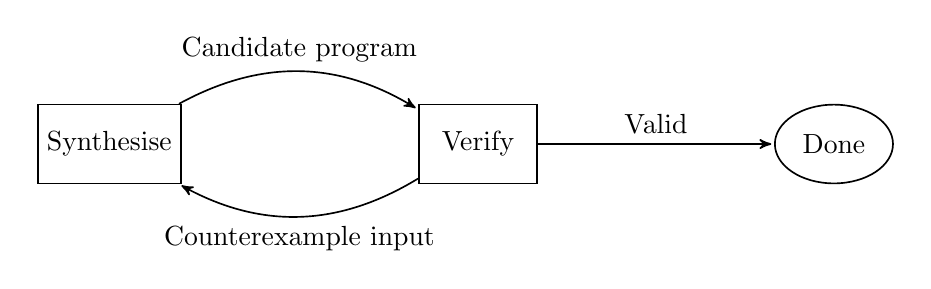
\begin{tikzpicture}[scale=0.5,->,>=stealth',shorten >=1pt,auto,
 semithick, initial text=]

  \matrix[nodes={draw, fill=none, scale=1, shape=rectangle, minimum height=1cm, minimum width=1.5cm},
          row sep=2cm, column sep=3cm] {
   \node (synth) {Synthesise};
   &
   \node (verif) {Verify}; %\\
   %\node[draw=none] {};
   &
   \node[ellipse] (done) {Done}; \\
  };

   \path
    (synth) edge [bend left] node {Candidate program} (verif)
    (verif) edge [bend left] node {Counterexample input} (synth)
    (verif) edge node {Valid} (done);
 \end{tikzpicture}
 
 \caption{Abstract synthesis refinement loop
 \label{fig:abstract-refinement}}
\end{figure*}

\iffalse
\subsection{The Concrete Algorithm for Bitvector Programs}
\label{sec:concrete-algorithm}

One area in which program synthesis can shine is in producing very small,
intricate programs that manipulate bitvectors.  An example of such a program
is given in Fig.~\ref{fig:bitvector-program}.  This program takes a machine word
as input and clears every bit except for the least significant bit that was set.
Even though this program is extremely short, it is fairly difficult for a human
to see what it does.  It is even more difficult for a human to come up with such
minimal code.  The program is so concise because it
takes advantage of the low-level details of the machine, such as the fact that
signed integers are stored in two's complement form.

\begin{figure*}
\centering
\begin{minipage}{0.45\linewidth}
 \begin{lstlisting}[language=C]
int isolate_lsb(int x) {
  return x & -x;
}
 \end{lstlisting}
\end{minipage}
\begin{minipage}{0.45\linewidth}
 
Example:

\hrule

\begin{tabular}{llcccccccc}
 x       & = & 1 & 0 & 1 & 1 & 1 & 0 & 1 & 0 \\
 -x      & = & 0 & 1 & 0 & 0 & 0 & 1 & 1 & 0 \\
 x \& -x & = & 0 & 0 & 0 & 0 & 0 & 0 & 1 & 0
\end{tabular}
\end{minipage}


 \caption{A tricky bitvector program}
  \label{fig:bitvector-program}
\end{figure*}


To synthesise tricky bitvector programs like this, it is natural for us to
work in the logic of quantifier-free propositional formulae and to use a
propositional SAT or SMT-$\mathcal{BV}$ solver as the decision procedure. 
However we propose a slightly different tack, which is to use a decidable
fragment of C as a ``high level'' logic.
\fi



%% To instantiate the abstract synthesis algorithm in \newC we must express $I, O,
%% \sigma$ and $P$ in \newC, then ensure that we can express the validity of the
%% synthesis formula as a safety property of the resulting \newC program.

%% Our encoding is the following:
%% %
%% \begin{itemize}
%%  \item $I$ is the set of $N$-tuples of 32-bit bitvectors.  This is written in \newC as the type \verb|int[N]|.
%%  \item $O$ is the set of $M$-tuples of 32-bit bitvectors, which is written in \newC as the type \verb|int[M]|.
%%  \item $\sigma$ is a pure function with type $I \times O \rightarrow \mathrm{Bool}$.  The \newC signature of this function is
%%  \verb|int check(int in[N], int out[M])|. This function is the only component supplied
%%  by the user.
%%  \item $P$ is written in a simple RISC-like language $\mathcal{L}$, whose syntax is given in Fig.~\ref{fig:l-language}.  Programs in $\mathcal{L}$
%%  have type $I \rightarrow O$ and
%%  are represented in \newC as objects of type \verb|prog_t|, shown in Fig.~\ref{fig:c-l-encoding}.
%%  \item We supply an interpreter for $\mathcal{L}$ which is written in \newC.  The type of
%%  this interpreter is $(I \rightarrow O) \times I \rightarrow O$ and the \newC signature is \\
%%  \verb|void exec(prog_t p, int in[N], int out[M])|.  Here, \verb|out| is an output parameter.
%% \end{itemize}

\begin{figure}
{\small
\begin{center}
\setlength{\tabcolsep}{16pt}
Integer arithmetic instructions:

\begin{tabular}{lll}
 \verb|add a b| & \verb|sub a b| & \verb|mul a b| \\
 \verb|neg a| & \verb|div a b|  & 
\end{tabular}

\medskip

Bitwise logical and shift instructions:

\begin{tabular}{lll}
 \verb|and  a b| & \verb|or a b| & \verb|xor a b| \\
 \verb|lshr a b| & \verb|ashr a b| & \verb|not  a| 
\end{tabular}

\medskip

Unsigned and signed comparison instructions:

\begin{tabular}{lll}
 \verb|le  a b| & \verb|lt  a b| & \verb|sle  a b| \\
 \verb|slt a b| & &
\end{tabular}
\end{center}
}
 \caption{The language $\mathcal{L}$}
 \label{fig:l-language}
\end{figure}


%% The exact details of how we encode an $\mathcal{L}$-program are given in Sec.~\ref{sec:encode-l}.
%% We must now express the {\sc synth} and {\sc verif} formulae as safety properties
%% of \newC programs, which is given in Fig.~\ref{fig:c-synthverif}.

%% \begin{figure}
%% \centering
%% \begin{minipage}[t]{.45\textwidth}
%% \begin{lstlisting}[language=C++]
%% void synth() {
%%   prog_t p = nondet();
%%   int in[N], out[M];

%%   assume(wellformed(p));

%%   in = test1;
%%   exec(p, in, out);
%%   assume(check(in, out));
%%   ...
%%   in = testN;
%%   exec(p, in, out);
%%   assume(check(in, out));
  
%%   assert(false);
%% }
%% \end{lstlisting}
%% %\end{minipage}
%% %\hfill
%% %\begin{minipage}[t]{.45\linewidth}
%% \begin{lstlisting}[language=C++]
%% void verif(prog_t p) {
%%   int in[N] = nondet();
%%   int out[M];

%%   exec(p, in, out);
%%   assert(check(in, out));
%% }
%% \end{lstlisting}
%% \end{minipage}

%%  \caption{The {\sc synth} and {\sc verif} formulae expressed as a \newC program.}
%%  \label{fig:c-synthverif}
%% \end{figure}

In order to determine the validity of the {\sc synth} formula, we can
check the {\sc synth} program for safety.  The {\sc synth} program is a
\newC program, which means we can check its safety by invoking a Bounded
Model Checker, such as {\sc cbmc}.

In some cases, it is faster to use an explicit-state model checker rather
than a Bounded Model Checker.  This is particularly true when we are checking
the {\sc verif} formula, where we have observed that incorrect programs tend
to be incorrect on a large fraction of the input space.  Counterexamples
are then very easy to find by explicit enumeration of a few inputs.
Since \newC is a fragment of C, we can generate an explicit-state
model checker using the same source files that we pass to {\sc cbmc}
and adding a small function to enumerate possible inputs.
We can run the explicit-state model checker
in parallel with {\sc cbmc} and take the answer of whichever happens
to terminate first, stopping the other process.  This procedure is
depicted for {\sc synth} in Fig.~\ref{fig:synth-dfd}, and is similar for {\sc verif}.

\begin{figure}
\begin{center}
\tikzstyle{file}=[draw, text width=7.0em, text centered,
  minimum height=1.5em]
\tikzstyle{process} = [draw, minimum height=3em, circle]
\tikzstyle{line} = [draw, color=black, -latex']


\resizebox{\linewidth}{!}{
\begin{tikzpicture}[font=\sffamily]

\node [file] (synth) {\sc synth.c};
\path (synth.south)+(0.0, -0.5) node [file] (tests) {\sc tests.c};
\path (tests.south)+(0.0, -0.5) node [file] (interpreter) {\sc interpreter.c};
\path (interpreter.south)+(0.0, -0.5) node [file] (spec) {\sc spec.c};

\path (tests.east)+(2.0, -0.25) node [process] (merged) {merge};

\path (merged.east)+(2.0, 1.0) node [process] (cbmc) {\sc cbmc};
\path (merged.east)+(2.0, -1.0) node [process] (gcc) {\sc gcc};

\path (cbmc.east)+(2.5, -1.0) node [file] (out) {candidate program};

\path [line] (synth) -- (merged);
\path [line] (tests) -- (merged);
\path [line] (interpreter) -- (merged);
\path [line] (spec) -- (merged);

\path [line] (merged) -- (cbmc);
\path [line] (merged) -- (gcc);

\path [line] (cbmc) -- (out);
\path [line] (gcc) -- (out);

\end{tikzpicture}
}
\end{center}

\caption{Schematic diagram of {\sc synth}}
\label{fig:synth-dfd}
\end{figure}

%\subsubsection{Encoding an $\mathcal{L}$-Program in \newC}
%% \label{sec:encode-l}

%% \begin{figure}
%% \begin{lstlisting}[language=c++,mathescape]
%% typedef $\mathcal{BV}(4)$ op_t;                  // An opcode
%% typedef $\mathcal{BV}(w)$ word_t;                // An $\mathcal{L}$-word
%% typedef $\mathcal{BV}(\log_2 \lceil c+l+a \rceil)$ param_t;  // An operand

%% struct prog_t {
%%   op_t ops[$l$];          // The opcodes
%%   param_t params[$l$*2];  // The operands
%%   word_t consts[$c$];     // The program constants
%% }
%% \end{lstlisting}

%%  \caption{The \newC structure we use to encode an $\mathcal{L}$ program
%%   \label{fig:c-l-encoding}}
%% \end{figure}

%% The exact \newC encoding of an $\mathcal{L}$ program is shown in Fig.~\ref{fig:c-l-encoding}.
%% The \verb|prog_t| structure encodes a program, which is a sequence of instructions.
%% The parameter $a$ is the number of arguments the program takes.
%% The $i$th instruction has opcode \verb|ops[i]|, left operand \verb|params[i*2]| and
%% right operand \verb|params[i*2 + 1]|.  An operand refers to either a program constant,
%% a program argument or the result of a previous instruction, and its value
%% is determined at runtime as follows:
%% \[
%%  val(x) = \begin{cases}
%%            x < a & \text{the } x^{\text{th}} \text{ program argument} \\
%%            a \leq x < a+c & \mathtt{consts[} x-a \mathtt{]} \\
%%            x \geq a + c & \text{the result of instruction } (x - a - c)
%%           \end{cases}
%% \]


%% A program is well formed if
%% no operand refers to the result of an instruction that has not been computed yet, and if
%% each opcode is valid.  We add a well-formedness constraint of the form \verb|params[i] <= (a+c+2*i)|
%% for each instruction.  It should be noted that this requires a linear number of well-formedness
%% constraints.  If all of these constraints are satisfied, the program is well-formed in the sense.



\subsection{Parameterising the Program Space}

In order to search the space of candidate programs, we parametrise
the language~$\mathcal{L}$, inducing a lattice of progressively
more expressive languages.  We start by attempting to synthesise
a program at the lowest point on this lattice and increase the
parameters of~$\mathcal{L}$ until we reach a point at which
the synthesis succeeds.

As well as giving us an automatic search procedure, this parametrisation
greatly increases the efficiency of our system since languages
low down the lattice are very easy to decide safety for.  If a program
can be synthesised in a low-complexity language, the whole procedure
finishes much faster than if synthesis had been attempted in a
high-complexity language.

---
We require the user to supply a program specification written in C, but then
ask nothing more of her.  We parametrise the space of programs in such a way
that it can be explored automatically, rather than asking a human for hints.
Our program encoding generates an $\exists
\forall$ formula that is \emph{linear} in the length of the shortest program
satisfying the user's specification.  This formula is then checked for satisfiability
using the CEGIS algorithm.
---

We introduce a novel parametrisation of the programming language
used to express our synthesised programs.
This parametrisation allows us to efficiently explore the program space
without relying on human guidance and also ensures that our programs
are of minimal length.

Our tool is the first we are aware of that is able to effectively
synthesise floating-point programs.  We demonstrate this by
synthesising {\sc Fast2Sum} using Knuth's {\sc 2Sum}~\cite{taocp2} as
a specification.
------


We consider the following parameters:
\begin{itemize}
\item{Program Length: $l$}
%% The first parameter we introduce is program length, denoted by $l$.
%% At each iteration we synthesise programs of length exactly $l$.
%% We start with $l = 1$ and increment $l$ whenever we determine
%% that no program of length $l$ can satisfy the specification.  When we do
%% successfully synthesise a program, we are \emph{guaranteed that it
%% is of minimal length} since we have previously established that no
%% shorter program is correct.
\item{Word Width: $w$}
%% An $\mathcal{L}$-program runs on a virtual machine (the $\mathcal{L}$-machine) that
%% has its own set of parameters.  The only relevant parameter is
%% the \emph{word width} of the $\mathcal{L}$-machine, that is, the number of bits
%% in each internal register and immediate constant.  This parameter is denoted by
%% $w$.  The size of the final SAT problem generated by {\sc cbmc} scales
%% polynomially with $w$, since each intermediate C variable corresponds
%% to $w$ propositional variables.

%% It is often the case that a program which satisfies the specification
%% on an $\mathcal{L}$-machine with $w = k$ will continue to satisfy the
%% specification when run on a machine with $w > k$.  For example, the program
%% in Fig.~\ref{fig:bitvector-program} isolates the least-significant bit of a word.
%% This is true irrespective of the word size of the machine it is run on -- it will
%% isolate the least-significant bit of an 8-bit word just as well as it will a
%% 32-bit word.  An often successful strategy is to synthesise a program for an
%% $\mathcal{L}$-machine with a small word size and then to check whether the
%% same program is correct when run on an $\mathcal{L}$-machine with a
%% full-sized word.

%% The only wrinkle here is that we will sometimes synthesise a program containing
%% constants.  If we have synthesised a program with $w=k$,
%% the constants in the program will be $k$-bits wide.  To extend the program
%% to an $n$-bit machine (with $n > k$), we need some way of deriving $n$-bit-wide
%% numbers from $k$-bit ones.  We have several strategies for this and
%% just try each in turn.  Our strategies are shown in Fig.~\ref{fig:generalize}.
%% $\mathcal{BV}(v, n)$ denotes an $n$-bit wide bitvector holding the value $v$
%% and $b \cdotp c$ means the concatenation of bitvectors $b$ and $c$.

%% \begin{figure}

%% \centering
%% \begin{minipage}[t]{.45\textwidth}
%% \begin{eqnarray*}
%%  \bv{m}{m} & \rightarrow & \bv{n}{n} \\
%%  \bv{m-1}{m} & \rightarrow & \bv{n-1}{n} \\
%%  \bv{m+1}{m} & \rightarrow & \bv{n+1}{n}
%% \end{eqnarray*}
%% \end{minipage}
%% \begin{minipage}[t]{.45\textwidth}
%% \begin{eqnarray*}
%%  \bv{x}{m} & \rightarrow & \bv{x}{n} \\
%%  \bv{x}{m} & \rightarrow & \bv{x}{m} \cdotp \bv{0}{n - m} \\
%%  \bv{x}{m} & \rightarrow & \underbrace{\bv{x}{m} \cdotp \ldots \cdotp \bv{x}{m}}_{\frac{n}{m} \mathrm{ times}}
%% \end{eqnarray*}
%% \end{minipage}

%% \caption{Rules for extending
%% an $m$-bit wide number to an $n$-bit wide one.
%%  \label{fig:generalize}}
%% \end{figure}

%% Sometimes a program will be correct for some particular word width $w$, but is
%% not correct for $w' > w$ even if the constants are replaced with appropriate ones.
%% When we detect this situation, we increase $w$ and continue synthesising.

\item{Number of Constants: $c$}
%% Instructions in $\mathcal{L}$ take either one or two operands.
%% Since any instruction whose operands are all constants can always be
%% eliminated (since its result is a constant), we know that a loop-free program
%% of minimal length will not contain any instructions with two constant
%% operands.  Therefore the number of constants that can appear in
%% a minimal program of length $l$ is at most $l$.  By minimising the number
%% of constants appearing in a program, we are able to use a particularly
%% efficient program encoding that speeds up the synthesis procedure
%% substantially.  The number of constants used in a program is the parameter $c$.

%% $\mathcal{L}$ is an SSA, three-address instruction set\footnote{
%% We experimented with implementing $\mathcal{L}$ as a stack machine, expecting
%% the programs to be smaller and synthesis to be faster as a result.  We saw
%% the opposite effect -- the more complex interpreter led to much slower synthesis.
%% }.  Destination registers
%% are implicit and a fresh register exists for each instruction to write its
%% output to.  A na\"{\i}ve way to encode $\mathcal{L}$ instructions is to have an
%% opcode and two operands, where each operand is either a register (i.e., a program argument
%% or the result of a previous instruction), or an immediate constant.

%% In this encoding, each opcode requires $\lceil \log_2 I \rceil$ bits to encode, where $I$ is the number
%% of instruction types in $\mathcal{L}$.  Each operand can be encoded using
%% $\log_2 w$ bits, where $w$ is the $\mathcal{L}$-machine word width, plus one
%% bit to specify whether the operand is a register name or an immediate constant.
%% One instruction can therefore be encoded using $\lceil \log_2 I \rceil + 2w + 2$ bits.
%% For an $n$-instruction program, we need $$\lceil n \log_2 I \rceil + 2nw + 2n$$ bits to encode
%% the entire program.

%% If we instead limit the number of constants that can appear in the program,
%% our operands can be encoded using fewer bits.  For an $n$-instruction program
%% using $c$ constants and taking $a$ arguments as inputs, each operand can refer
%% to a program argument, the result of a previous instruction or a constant.
%% This can be encoded using $\lceil \log_2 (c+a+n-1) \rceil$ bits, which means each instruction
%% can be encoded in $\lceil \log_2 I \rceil + \lceil \log_2 (c + a + n - 1) \rceil$ and the full program
%% needs $$\lceil n \log_2 I \rceil + \lceil n \log_2 (c + a + n - 1) \rceil + cw$$ bits to encode.

%% We give an example. Our language $\mathcal{L}$ has 15 instruction types, so each opcode is 4 bits.
%% For a 10-instruction program over 1 argument, using 2 constants on a 32-bit word
%% machine the first encoding requires $10 * (4 + 32 + 1 + 32 + 1) = 700$ bits.
%% Using the second encoding, each operand can be represented using
%% $\log_2 (2 + 1 + 10 - 1) = 4$ bits, and the entire program requires 184 bits.
%% This is a substantial reduction in size and when the desired program requires
%% only few constants this can lead to a very significant speed up.

%% As with program length, we progressively increase the number of constants in
%% our program.  We start by trying to synthesise a program with no constants,
%% then if that fails we attempt to synthesise using one constant and so on until we
%% reach $c = l$.

\end{itemize}
\subsubsection{Searching the Program Space}

The key to our automation approach is to come up with a sensible way in which to
adjust the $\mathcal{L}$-parameters in order to cover all possible programs.
After each round of {\sc synth}, we may need to adjust the parameters.  The
logic for these adjustments is shown as a tree in Fig.~\ref{fig:paramsflow}.

Whenever {\sc synth} fails, we consider which parameter might have caused the
failure.  There are two possibilities: either the program length $l$ was too small,
or the number of allowed constants $c$ was.  If $c < l$, we just increment $c$ and
try another round of synthesis, but allowing ourselves an extra program constant.
If $c = l$, there is no point in increasing $c$ any further.  This is because
no minimal $\mathcal{L}$-program has $c > l$, for if it did there would
have to be at least one instruction with two constant operands.  This
instruction could be removed (at the expense of adding its result as
a constant), contradicting the assumed minimality of the program.  So
if $c = l$, we set $c$ to 0 and increment $l$, before attempting
synthesis again.

If {\sc synth} succeeds but {\sc verif} fails, we have a candidate
program that is correct for some inputs but incorrect on at least
one input.  However, it may be the case that the candidate program
is correct for \emph{all} inputs when run on an $\mathcal{L}$-machine
with a small word size.  For example, we may have synthesised a
program which is correct for all 8-bit inputs, but incorrect for
some 32-bit input.  If this is the case (which we can determine
by running the candidate program through {\sc verif} using the smaller
word size), we may be able to produce a correct program for
the full $\mathcal{L}$-machine by using the constant extension rules
shown in Fig.~\ref{fig:generalize}.  If constant generalization
is able to find a correct program, we are done.  Otherwise,
we need to increase the word width of the $\mathcal{L}$-machine
we are currently synthesising for.

%% \begin{figure}[t]
%% \centering
%% \begin{tikzpicture}[scale=0.65, transform shape, node distance=2cm, auto]
%% \tikzstyle{decision} = [diamond, draw, fill=blue!20, 
%%     text width=4.5em, text badly centered, node distance=3cm, inner sep=0pt]
%% \tikzstyle{block} = [rectangle, draw, fill=blue!20, 
%%     text width=5em, text centered, rounded corners, minimum height=4em]
%% \tikzstyle{line} = [draw, -latex']
%% \tikzstyle{cloud} = [draw, ellipse,fill=red!20, node distance=3cm,
%%     minimum height=2em]

%%  \node [decision] (synthsucc) {{\sc Synth} succeeds?};

%%  \node [decision, below of=synthsucc, node distance=2.5cm] (verif) {{\sc Verif} succeeds?};
%%  \node [decision, right of=verif] (ck) {$c < l$?};

%%  \node [block, below of=verif, node distance=3cm]   (done) {Done!};
%%  \node [decision, left of=verif] (verifw) {{\sc Verif} succeeds for small words?};

%%  \node [block, below of=ck, node distance=2.5cm] (incc) {$c := c+1$};
%%  \node [block, right of=incc, node distance=2cm] (incl) {$c := 0$\\ $l := l+1$};

%%  \node [decision, below of=verifw, node distance=3cm] (gen) {Extend succeeds?};
%%  \node [block, left of=verifw, node distance=3cm] (iterate) {Parameters unchanged};

%%  \node [block, left of=gen, node distance=3cm] (incw) {$w := w+1$};

%%  \path [line] (synthsucc) -- node [left] {Yes} (verif);
%%  \path [line] (synthsucc) -| node [above, near start] {No} (ck);

%%  \path [line] (verif) -- node [left] {Yes} (done);
%%  \path [line] (verif) -- node [above, near start] {No} (verifw);

%%  \path [line] (ck) -- node [left] {Yes} (incc);
%%  \path [line] (ck) -| node  [above, near start]  {No} (incl);

%%  \path [line] (verifw) -- node [right] {Yes} (gen);
%%  \path [line] (verifw) -- node [above] {No} (iterate);
 
%%  \path [line] (gen) -- node [below] {Yes} (done);
%%  \path [line] (gen) -- node [below] {No} (incw);

%%  %\path [dotted, line] (iterate.west) |- (synthsucc);
%% \end{tikzpicture}

%%  \caption{Decision tree for increasing parameters of $\mathcal{L}$.}
%%  \label{fig:paramsflow}

%% \end{figure}

\iffalse

\subsection{Implementation Issues}
For performance reasons, we found that adding extra constraints on the
syntax of the synthesised programs sped up synthesis.  The extra constraints
fell into two categories: eliminating nops and instruction-level symmetry reduction.

\subsubsection{Remove nops}
Many instructions in $\mathcal{L}$ are nops that do not doing anything,
for example the instruction \verb|add x 0|.  Such instructions
can be removed from any program they appear in to leave a semantically
equivalent, but shorter, program.  We can therefore be sure that nops
will never appear in any minimal program.  By adding constraints saying that
each instruction is not a nop, we can help the underlying SAT solver's
search, which reduces the runtime of the overall procedure.

\subsubsection{Symmetry Reduction}
There are many instructions that are equivalent to each other.  For example,
\verb|add x y| is equivalent to \verb|add y x| -- any program containing
one instruction could have it replaced by the other instruction and
keep the same semantics.  We choose a single canonical instruction to
represent all instructions in a particular equivalence class, then add
constraints saying that no non-canonical instructions appear in the program.

Our rules for excluding non-canonical instructions are:

\begin{itemize}
 \item For commutative operations, the first operand is smaller than the second.
 \item For unary operations, the second (unused) operand is always 0.
 \item No instruction may have two constant operands.
 \item All constants in the constant table are distinct.
\end{itemize}

As with the nop constraints, these additional constraints do increase the
size of the resulting SAT instance, but this still ends up as a win in
terms of runtime.
\fi

\iffalse
\section{Experiments}
\label{sec:experiments}
\subsection{Experimental Setup}
We implemented our fully automatic synthesis procedure as the {\sc kalashnikov} tool.  The implementation consists
of around 600 lines of \newC and 600 lines of Python.  To evaluate the tool we used the 29 bitvector
programs from~\cite{brahma} and~\cite{brahma-icse}.  The majority of these are ``bit twiddling hacks'' taken from
Hacker's Delight~\cite{hackers-delight}.  The code we used to perform the experiments, along with the
benchmarks, is available at \texttt{http://www.cprover.org/kalashnikov} and the benchmarks can also
be found in Appendix~\ref{app:benchmarks}.  As a backend solver, we used
{\sc CBMC}~\cite{cbmc-website} at SVN revision r3545, with Glucose 3.0~\cite{glucose-paper} as the SAT solver.
We performed our experiments on a 4-core, 2.40\,GHz Xeon E5-2665 with 32\,GB of RAM.

To give a reference point for the efficiency of our tool, we present the results given for {\sc brahma}
on the same benchmarks, as reported in~\cite{brahma} and~\cite{brahma-icse}.
These experiments were performed on an 8-core,
1.86\,GHz Xeon with 4\,GB of RAM.

Since we were unable to obtain a copy of {\sc brahma}, we re-implemented the {\sc brahma} program encoding in our framework,
resulting in the {\sc brahmikov} tool. {\sc Brahmikov} implements the component based synthesis
paradigm, but still uses {\sc cbmc} as the backend decision procedure.  Since {\sc brahma} and {\sc brahmikov} are written in
different frameworks, we cannot compare their performance.  However we can compare {\sc brahmikov} and {\sc kalashnikov}.
In particular it is interesting to note that {\sc brahmikov} often produces longer programs than {\sc kalashnikov}.  We
believe this is due to differences in the post-processing strategies used by {\sc brahmikov} and {\sc brahma}.  {\sc Brahmikov}
performs syntatic dead code elimination (following~\cite{brahma}), but this is not enough to generate minimal programs
in many cases.  This is in contrast to {\sc kalashnikov}, which always generates minimal programs.

We also ran the {\sc AHA} superoptimiser on our benchmarks and found that on the small problems
(those with 2-instruction solutions)
{\sc AHA} found a single correct solution in negligible time.  On the larger benchmarks, candidate solutions
were still found rapidly (around 10\,s for the 3-instruction programs) but the number of candidates was
too large to practically check them all.  For example, {\sc AHA} found 2284262 candidate
programs in 12.13\,s for p12.

We invested significant effort into trying to implement the benchmarks in a way
that would allow us to compare with {\sc sketch}. Unfortunately, we were unable to come up
with an encoding that afforded a meaningful comparison.  In retrospect,
we realise that this is due to a fundamental difference in the problem domains
our respective tools are designed to solve: {\sc sketch} is able to use
human insight to generate large, complex programs, whereas we are optimised for 
automatically generating small programs with somewhat more intricate data-flow.


\subsection{Results and Analysis}
The results of our experiments are shown in Fig.~\ref{fig:results-table}.
Column 1 shows the runtime reported for each benchmark in \cite{brahma}, column 2
shows the number of instructions in the synthesised program, and column 3 contains a \xmark\;when
{\sc Brahma} needed user assistance to solve a benchmark.
Columns 4 through 7 show the same information, but with the data taken from~\cite{brahma-icse}.
Column 5 shows the runtimes for the version of {\sc Brahma} from~\cite{brahma-icse} which
implemented the semibiased optimisation.
Finally, columns 8 and 10 show the runtime for {\sc Brahmikov} and {\sc Kalashnikov} respectively.
Columns 9 and 11 show the number of instructions
in the program synthesised by {\sc Brahmikov} and {\sc Kalashnikov}.  In all cases,
{\sc Brahmikov} performs very poorly, which demonstrates that the {\sc Kalashnikov} program
encoding is more suitable for our system than the component based synthesis encoding.
We also ran the {\sc Brahmikov} experiments using Z3 as the solver rather than Glucose,
but this configuration failed to terminate for any of the examples.

The results can be divided into three categories, as follows:


\paragraph{\bf {\sc Kalashnikov} synthesises a shorter program than {\sc Brahma}:}
This happens in 4 of the 29 cases, which is to be expected since {\sc Kalashnikov}'s outputs
are, by construction, guaranteed to be minimal.  This case is illustrated by benchmark p29, shown in Fig.~\ref{fig:obfuscated}.
The specification here is a piece of obfuscated code taken from the Conficker worm~\cite{conficker}, and
our goal is to synthesise an equivalent program which is easier to understand.  The obfuscated code
uses several tricks, including an apparently unbounded loop.  {\sc Brahma} is able to
produce an equivalent program consisting of four instructions using shifts and addition, whereas {\sc kalashnikov}
is able to produce the minimal program \verb|y * 45|.  It is also worth noting that the specification
fed to {\sc kalashnikov} was just the obfuscated code, with no further preprocessing needed.
\paragraph{\bf {\sc Kalashnikov} is unable to synthesise a program:}
This happens in 8 of the 29 cases.  In each case, {\sc Brahma} needs user guidance to synthesise the program.
The existence of instances that are beyond the reach of current automatic
methods, and thus require manual intervention, is to be expected.
% A total of 8 tests fall into this category.
\paragraph{\bf {\sc Brahma} and {\sc Kalashnikov} both synthesise minimal programs:}
In the remaining cases, both {\sc brahma} and {\sc kalashnikov} are able to produce
minimal programs.  It was not clear from just looking at the runtime numbers whether
any of the tools was significantly faster than the others, so we performed a Wilcoxon signed-rank test.

For each pair of tools ({\sc kalashnikov} vs. each of the {\sc brahma} configurations), the Wilcoxon test was
unable to reject the null hypothesis (that the tools are equally fast) at the p=0.05 level. In other words,
there is no statistically significant difference in the speed of {\sc kalashnikov} and {\sc brahma}.

\begin{figure}
Obfuscated code

\begin{lstlisting}[frame=single,language=c]
int obfuscated (int y) {
 int a=1, b=0, z=1, c=0;
 while(1) {
  if (a == 0) { if (b == 0) { y=z+y; a =!a; b=!b;c=!c;
  if (!c) break;} else { z=z+y; a=!a; b=!b; c=!c;
  if (!c) break;} } else { if (b == 0) { z=y << 2;
  a=!a; } else { z=y << 3; a=!a; b=!b; } }
 }
 return z;
}
\end{lstlisting}
%\end{minipage}

\begin{minipage}[t]{.45\textwidth}
{\sc Brahma}'s output

\begin{lstlisting}[language=c,frame=single]
int recovered (int y) {
 int z = y << 2;
 y = z + y;
 z = y << 3
 y = z + y;
 return z;
}
\end{lstlisting}
\end{minipage}
\hfill
\begin{minipage}[t]{.45\textwidth}
{\sc Kalashnikov}'s output
 \begin{lstlisting}[language=c,frame=single]
int recovered (int y) {
 return y*45;
}
\end{lstlisting}
\end{minipage}

 \caption{De-obfuscating  C code.
  \label{fig:obfuscated}}
\end{figure}

\subsection{Floating Point}
To demonstrate the capabilities of \newC as an implementation language, we synthesise a
non-trivial floating-point program.  For this we chose the classic {\sc 2Sum} algorithm for computing
exact sums of floating-point numbers.  The original {\sc 2Sum} algorithm is given as Alg.~\ref{alg:2sum}.
In the case that $a \ge b$, exact addition can be implemented in fewer instructions -- this is the
{\sc Fast2Sum} algorithm~\cite{fast2sum}, shown in Alg.~\ref{alg:fast2sum}.  We used {\sc 2sum} as our specification, and
added an assumption that $a \ge b$.  {\sc Kalashnikov} is able to synthesise and verify the
code for {\sc Fast2Sum} from this specification in 396.07\,s, which we believe to be the first time
this has been achieved.  {\sc 2Sum} was proved to be minimal in~\cite{fast2sum}, but
we believe our synthesis constitutes the first proof that {\sc Fast2Sum} is
minimal under the assumption that $a \ge b$.

\begin{figure}[ht]
\begin{center}
\begin{minipage}[t]{0.45\linewidth}
\begin{algorithm}[H]
\caption{\sc 2Sum
 \label{alg:2sum}}
\begin{algorithmic}
\Let{$s$}{$a+b$}
\Let{$b'$}{$s - a$}
\Let{$a'$}{$s - b'$}
\Let{$\delta b$}{$b - b'$}
\Let{$\delta a$}{$a - a'$}
\Let{$t$}{$\delta a + \delta b$}
\Ensure{$a + b$ = $s + t$ exactly}
\end{algorithmic}
\end{algorithm}
\end{minipage}
\hfill
\begin{minipage}[t]{0.45\linewidth}
\begin{algorithm}[H]
\caption{\sc Fast2Sum
 \label{alg:fast2sum}}
\begin{algorithmic}
\Require{$a \ge b$}
\Let{$s$}{$a + b$}
\Let{$z$}{$s - a$}
\Let{$t$}{$b - z$}
\Ensure{$a + b$ = $s + t$ exactly}
\end{algorithmic}
\end{algorithm}
\end{minipage}
\end{center}


 \caption{The {\sc 2Sum} algorithm for correctly rounded floating-point sums.}
  \label{fig:2sum}
\end{figure}

\begin{figure}[ht]
\centering
{\tiny
\begin{tabular}{l||rrc|rrrc|rr|rr}
Problem & \multicolumn{3}{c}{\sc PLDI Brahma} & \multicolumn{4}{|c}{ICSE Brahma} & \multicolumn{2}{|c}{\sc Brahmikov} & \multicolumn{2}{|c}{\sc Kalashnikov} \\
        & Runtime & \#Lines & Aut. & Random & Semibiased & \#Lines & Aut. & Runtime & \#Lines & Runtime & \#Lines \\
\hline
\hline
p1 & 3.20s &{\bf 2} & & 1.48s & {\bf 0.80s} & {\bf 2} & & 117.02s &5 &2.71s &{\bf 2} \\
p2 & 3.60s &{\bf 2} & & 7.35s & 4.75s & {\bf 2} & & 46.38s &4 &{\bf 2.24s} &{\bf 2} \\
p3 & 1.40s &{\bf 2} & & 1.60s & {\bf 0.65s} & {\bf 2} & & 131.06s &6 &1.92s &{\bf 2} \\
p4 & 3.30s &{\bf 2} & & 1.65s & {\bf 0.86s} & {\bf 2} & & 52.13s &7 &2.71s &{\bf 2} \\
p5 & {\bf 2.20s} &{\bf 2} & & 3.92s & 2.28s & {\bf 2} & & 73.60s &{\bf 2} &2.77s &{\bf 2} \\
p6 & 2.40s &{\bf 2} & & 6.22s & {\bf 1.64s} & {\bf 2} & & 41.95s &3 &2.23s &{\bf 2} \\
p7 & 1.00s &{\bf 3} & & 1.39s & {\bf 0.50s} & {\bf 3} & & 166.56s &{\bf 3} &6.38s &{\bf 3} \\
p8 & {\bf 1.40s} &{\bf 3} & & 2.20s & 1.42s & {\bf 3} & & 86.30s &{\bf 3} &6.73s &{\bf 3} \\
p9 & 5.80s &{\bf 3} & & {\bf 4.95s} & 8.75s & {\bf 3} & \xmark & 524.77s &7 &15.14s &{\bf 3} \\
p10 & 76.10s &{\bf 3} & & 13.99s & {\bf 7.82s} & {\bf 3} & \xmark & T/O &-- &18.59s &{\bf 3} \\
p11 & 57.10s &{\bf 3} & & 24.31s & 17.13s & {\bf 3} & \xmark & T/O &-- &{\bf 15.17s} &{\bf 3} \\
p12 & 67.80s &{\bf 3} & & 279.49s & 48.16s & {\bf 3} & \xmark & 534.26s &5 &{\bf 16.21s} &{\bf 3} \\
p13 & {\bf 6.20s} &4 & & 32.50s & 9.97s & 4 & \xmark & 255.22s &10 &12.56s &{\bf 3} \\
p14 & 59.60s &{\bf 4} & & 167.84s & {\bf 18.07s} & {\bf 4} & \xmark & T/O &-- &81.87s &{\bf 4} \\
p15 & 118.90s &{\bf 4} & & 228.78s & {\bf 33.53s} & {\bf 4} & \xmark & T/O &-- &104.97s &{\bf 4} \\
p16 & 62.30s &{\bf 4} & & 66.93s & {\bf 23.92s} & {\bf 4} & \xmark & T/O &-- &49.90s &{\bf 4} \\
p17 & 78.10s &{\bf 4} & & 163.82s & 65.45s & {\bf 4} & & 488.92s &9 &{\bf 56.56s} &{\bf 4} \\
p18 & 45.90s &6 & \xmark & 214.14s & 82.53s & 6 & \xmark & 311.58s &8 &{\bf 8.71s} &{\bf 3} \\
p19 & {\bf 34.70s} &6 & \xmark & N/A & N/A &-- & & T/O &-- &T/O &-- \\
p20 & {\bf 108.40s} &7 & \xmark & 1074.04s & 285.56s & 7 & \xmark & T/O &-- &T/O &-- \\
p21 & {\bf 28.30s} &8 & \xmark & N/A & N/A &-- & & T/O &-- &T/O &-- \\
p22 & {\bf 279.00s} &8 & \xmark & N/A & N/A &-- & & T/O &-- &T/O &-- \\
p23 & {\bf 1668.00s} &10 & \xmark & N/A & N/A &-- & & T/O &-- &T/O &-- \\
p24 & {\bf 224.90s} &12 & \xmark & T/O & 372.74s & 12 & \xmark & T/O &-- &T/O &-- \\
p25 & {\bf 2778.70s} &16 & \xmark & N/A & N/A &-- & & T/O &-- &T/O &-- \\
p26 & N/A &-- & & 14.32s & 6.66s & 4 & \xmark & T/O &-- &{\bf 1.47s} &{\bf 1} \\
p27 & N/A &-- & & 217.34s & {\bf 26.51s} & {\bf 4} & \xmark & T/O &-- &54.28s &{\bf 4} \\
p28 & N/A &-- & & {\bf 1.38s} & 24.24s & 3 & \xmark & T/O &-- &1.80s &{\bf 2} \\
p29 & N/A &-- & & {\bf 5.28s} & 5.92s & 4 & \xmark & T/O &-- &8.78s &{\bf 1} \\
\end{tabular}

}
\caption{Time for synthesis of machine integer benchmarks from~\cite{brahma} and~\cite{brahma-icse}.
 \label{fig:results-table}}
\end{figure}

%\begin{figure}[p]
%\begin{center}
%{\tiny
%\begin{tabular}{l||rr|rr|rr}
Problem & \multicolumn{2}{c}{Random {\sc Brahma}} & \multicolumn{2}{|c}{Semibiased {\sc Brahma}} & \multicolumn{2}{|c}{\sc Kalashnikov} \\
        & Runtime & \#Lines & Runtime & \#Lines & Runtime & \#Lines \\
\hline
\hline
p1 & 1.48s &2 &{\bf 0.80s} &2 &1.83s &2 \\
p2 & 7.35s &2 &4.75s &2 &{\bf 1.49s} &2 \\
p3 & 1.60s &2 &{\bf 0.65s} &2 &1.60s &2 \\
p4 & 1.65s &2 &{\bf 0.86s} &2 &1.86s &2 \\
p5 & 3.92s &2 &2.28s &2 &{\bf 1.98s} &2 \\
p6 & 6.22s &2 &1.64s &2 &{\bf 1.51s} &2 \\
p7 & 1.39s &3 &{\bf 0.50s} &3 &4.04s &3 \\
p8 & 2.20s &3 &{\bf 1.42s} &3 &4.31s &3 \\
p9 & {\bf 4.95s} &3 &8.75s &3 &5.74s &3 \\
p10 & 13.99s &3 &{\bf 7.82s} &3 &9.80s &3 \\
p11 & 24.31s &3 &17.13s &3 &{\bf 9.40s} &3 \\
p12 & 279.49s &3 &48.16s &3 &{\bf 10.12s} &3 \\
p13 & 32.50s &4 &{\bf 9.97s} &4 &10.24s &{\bf 3} \\
p14 & 14.32s &4 &{\bf 6.66s} &4 &-- &-- \\
p15 & 167.84s &4 &{\bf 18.07s} &4 &40.28s &4 \\
p16 & 66.93s &4 &{\bf 23.92s} &4 &27.41s &4 \\
p17 & 217.34s &4 &{\bf 26.51s} &4 &41.37s &4 \\
p18 & 228.78s &4 &{\bf 33.53s} &4 &35.02s &4 \\
p19 & 163.82s &4 &65.45s &4 &{\bf 27.73s} &4 \\
p20 & 214.14s &6 &82.53s &6 &{\bf 5.55s} &{\bf 3} \\
p21 & 1074.04s &7 &{\bf 285.56s} &7 &-- &-- \\
p22 & -- &-- &{\bf 372.74s} &12 &-- &-- \\
p23 & 1.38s &3 &12.12s &3 &{\bf 1.20s} &{\bf 2} \\
p24 & 5.28s &4 &{\bf 2.96s} &4 &4.64s &{\bf 1} \\
\end{tabular}

%}
%\end{center}
%\caption{Times for synthesis of machine integer benchmarks from~\cite{brahma-icse}.}
%\label{fig:icse-results-table}
%\end{figure}



\section{Conclusion}

By expressing the program synthesis problem as a safety property for a
program interpreter, we have been able to harness the power of
state-of-the-art program analysis tools and reuse them in a new problem
domain.  We have implemented our algorithm as a freely downloadable tool
whose performance compares favourably to a recent program synthesiser. 
Finally, we have taken advantage of the expressiveness of our specification
language to make an initial step towards practical synthesis of
floating-point programs.

\paragraph{Future Work}

It may be possible to extend the language $\mathcal{L}$ with constructs such
as branching and limited looping while still retaining decidability, which
would be an interesting direction to pursue.  Since our specification
language is a subset of C, it is straight-forward to interface {\sc
kalashnikov} with other analysis tools.  Various problems such as ranking
function synthesis, loop invariant generation and loop
summarisation can be phrased as program synthesis problems, and we would like to investigate the
possibilities of applying {\sc kalashnikov} to these domains.

\paragraph{Acknowledgements}
We thank Martin Brain for his insight and advice during our synthesis discussions.
Also, thanks to Cristina David for her extensive help and proofreading during the
preparation of this paper.

\bibliography{synth}{}
\bibliographystyle{splncs}

\appendix

\section{Benchmarks}
\label{app:benchmarks}

\begin{figure}
\scriptsize
 \begin{multicols}{4}
 
   \begin{minipage}{.2\textwidth}
   \bf{P1}($x$): Turn-off rightmost 1 bit.
   \begin{enumerate}
    \item $t1 = x - 1$
    \item $t2 = x \& t1$
   \end{enumerate}
   \end{minipage}

   \vspace{12pt}
   
   \begin{minipage}{.2\textwidth}
   \bf{P2}($x$): Test whether $x$ is of the form $2^n - 1$.
   \begin{enumerate}
    \item $t1 = x + 1$
    \item $t2 = x \& t1$
   \end{enumerate}
   \end{minipage}

   \vspace{12pt}
   

   \begin{minipage}{.2\textwidth}
   \bf{P3}($x$): Isolate the rightmost 1 bit.
   \begin{enumerate}
    \item $t1 = -x$
    \item $t2 = x \& t1$
   \end{enumerate}
   \end{minipage}

   \vspace{12pt}
   

   \begin{minipage}{.2\textwidth}
   \bf{P4}($x$): Form a mask that identifies the rightmost 1 bit and trailing 0s.
   \begin{enumerate}
    \item $t1 = x - 1$
    \item $t2 = x \oplus t1$
   \end{enumerate}
   \end{minipage}

   \vspace{12pt}
   
   \begin{minipage}{.2\textwidth}
   \bf{P5}($x$): Right propagate the rightmost 1 bit.
   \begin{enumerate}
    \item $t1 = x - 1$
    \item $t2 = x \mid t1$
   \end{enumerate}
   \end{minipage}

   \vspace{12pt}
   
   \begin{minipage}{.2\textwidth}
   \bf{P6}($x$): Turn on the rightmost 0 bit.
   \begin{enumerate}
    \item $t1 = x + 1$
    \item $t2 = x \mid t1$
   \end{enumerate}
   \end{minipage}
      \vspace{12pt}
   
   \begin{minipage}{.2\textwidth}
   \bf{P7}($x$): Isolate the rightmost 0 bit.
   \begin{enumerate}
    \item $t1 = \sim x$
    \item $t2 = x + 1$
    \item $t3 = t1 \& t2$
   \end{enumerate}
   \end{minipage}
   \vspace{12pt}
   
   \begin{minipage}{.2\textwidth}
   \bf{P8}($x$): Form a mask the identifies the trailing 0s.
   \begin{enumerate}
    \item $t1 = x -1$
    \item $t2 = \sim x$
    \item $t3 = t1 \& t2$
   \end{enumerate}
   \end{minipage}
   \vspace{12pt}
   
   \begin{minipage}{.2\textwidth}
   \bf{P9}($x$): Absolute value.
   \begin{enumerate}
    \item $t1 = x >> 31$
    \item $t2 = x \oplus t1$
    \item $t3 = t2 - t1$
   \end{enumerate}
   \end{minipage}

      \vspace{12pt}
   
   \begin{minipage}{.2\textwidth}
   \bf{P10}($x, y$): Test if nlz(x) == nlz(y), where nlz is number of leading zeroes.
   \begin{enumerate}
    \item $t1 = x \& y$
    \item $t2 = x \oplus y$
    \item $t3 = t2 \leq t1$
   \end{enumerate}
   \end{minipage}

   
      \vspace{12pt}
   
   \begin{minipage}{.2\textwidth}
   \bf{P11}($x, y$): Test if nlz(x) < nlz(y).
   \begin{enumerate}
    \item $t1 = \sim y$
    \item $t2 = x \& t1$
    \item $t3 = t2 > y$
   \end{enumerate}
   \end{minipage}
   \vspace{12pt}
   
   \begin{minipage}{.2\textwidth}
   \bf{P12}($x, y$): Test if nlz(x) <= nlz(y).
   \begin{enumerate}
    \item $t1 = \sim y$
    \item $t2 = x \& t1$
    \item $t3 = t2 \leq y$
   \end{enumerate}
   \end{minipage}
   
      \vspace{12pt}
   
   \begin{minipage}{.2\textwidth}
   \bf{P13}($x$): Sign.
   \begin{enumerate}
    \item $t1 = x >> 31$
    \item $t2 = t1 < x$
    \item $t3 = t2 + t1$
   \end{enumerate}
   \end{minipage}

   \vspace{12pt}

   \begin{minipage}{.2\textwidth}
   \bf{P14}($x, y$): Floor of average of $x$ and $y$ without overflowing.
   \begin{enumerate}
    \item $t1 = x \& y$
    \item $t2 = x \oplus y$
    \item $t3 = t2 >> 1$
    \item $t4 = t1 + t3$
   \end{enumerate}
   \end{minipage}
   \vspace{12pt}
   
   \begin{minipage}{.2\textwidth}
   \bf{P15}($x, y$): Ceil of average of $x$ and $y$ without overflowing.
   \begin{enumerate}
    \item $t1 = x \mid y$
    \item $t2 = x \oplus y$
    \item $t3 = t2 >> 1$
    \item $t4 = t1 - t3$
   \end{enumerate}
   \end{minipage}
   \vspace{12pt}
   
   \begin{minipage}{.2\textwidth}
   \bf{P16}($x$): Max.
   \begin{enumerate}
    \item $t1 = x \leq y$
    \item $t2 = x \oplus y$
    \item $t3 = t1 * t2$
    \item $t4 = t3 \oplus y$
   \end{enumerate}
   \end{minipage}
   \vspace{12pt}
   
   \begin{minipage}{.2\textwidth}
   \bf{P17}($x$): Turn off the rightmost contiguous string of 1 bits.
   \begin{enumerate}
    \item $t1 = x - 1$
    \item $t2 = x \mid t1$
    \item $t3 = t2 + 1$
    \item $t4 = t3 \& x$
   \end{enumerate}
   \end{minipage}
   \vspace{12pt}
   
   \begin{minipage}{.2\textwidth}
   \bf{P18}($x$): Determine if $x$ is a power of 2.
   \begin{enumerate}
    \item $t1 = -x$
    \item $t2 = x \oplus t1$
    \item $t3 = t2 < t1$
   \end{enumerate}
   \end{minipage}
   \vspace{12pt}
  
   
   
   \begin{minipage}{.2\textwidth}
   {\bf P19($x, m, k$): Exchange two fields of $x$, demarcated by $m$ and $k$.}

   N/A ({\sc Kalashnikov} was unable to synthesise this program.)
   \end{minipage}
   \vspace{12pt}
   
   \begin{minipage}{.2\textwidth}
   {\bf P20($x$): Next higher unsigned number with the same number of 1 bits.}

   N/A
   \end{minipage}
   \vspace{12pt}
   
   \begin{minipage}{.2\textwidth}
   {\bf P21($x, a, b, c$): Cycling through 3 values $a, b, c$.}

    N/A
   \end{minipage}
   \vspace{12pt}
   
   \begin{minipage}{.2\textwidth}
   {\bf P22($x$): Compute parity.}

    N/A
   \end{minipage}
   \vspace{12pt}
   
   \begin{minipage}{.2\textwidth}
   {\bf P23($x$): Count number of set bits.}

    N/A
   \end{minipage}
      \vspace{12pt}
   
   \begin{minipage}{.2\textwidth}
   {\bf P24($x$): Round up to next highest power of 2.}

    N/A
   \end{minipage}
   \vspace{12pt}
   
   \begin{minipage}{.2\textwidth}
   {\bf P25($x, y$): Computer higher order half of $x \times y$.}

    N/A
   \end{minipage}

   \vspace{12pt}

   \begin{minipage}{.2\textwidth}
   {\bf P26($x, k$): Round $x$ up to a multiple of $2^k$.}

N/A
   \end{minipage}

      \vspace{12pt}
   
   \begin{minipage}{.2\textwidth}
   {\bf P27($x, y$): Min.}
    \begin{enumerate}
     \item $t1 = x \oplus y$
     \item $t2 = t1 \leq t2$
     \item $t3 = t1 * t2$
     \item $t4 = y \oplus t3$
    \end{enumerate}
   \end{minipage}

   
 \end{multicols}

 \caption{The integer benchmarks}
\end{figure}

\begin{figure}
 \begin{lstlisting}[language=C++]
void interchangeObs(word_t* src, word_t* dest)
{
  *src = *src ^ *dest;

  if (*src == (*src ^ *dest)) {
    *src = *src ^ *dest;

    if (*src == (*src ^ *dest)) {
      *dest = *src ^ *dest;
      
      if (*dest == (*src ^ *dest)) {
        *src = *dest ^ *src;
        return;
      } else {
        *src = *src ^ *dest;
        *dest = *src ^ *dest;
        return;
      } 
    } else
      *src = *src ^ *dest;
  }
  
  *dest = *src ^ *dest;
  *src = *src ^ *dest;

  return;
}
 \end{lstlisting}

 \caption{Benchmark 28: an obfuscated swap function}
\end{figure}

\begin{figure}
 \begin{lstlisting}[language=C++]
int mul45(int y) {
  int a=1, b=0, z=1, c=0;

  while(1) {
    if (a == 0) {
      if (b == 0) {
	y=z+y; a =!a; b=!b;c=!c;
	if (! c) break;
      } else {
	z=z+y; a=!a; b=!b; c=!c;
	if (! c) break;
      }
    } else {
      if (b == 0) { z=y << 2; a=!a; }
      else {
	z=y << 3; a=!a; b=!b; } } }

  return y;
}
	
 \end{lstlisting}

 \caption{Benchmark 29: an obfuscated function to multiply by 45}
 
\end{figure}

\fi


\section{Genetic Programming and Incremental Evolution}

We begin by observing that the asymptotic complexity of all of our synthesis
backends are equal, assuming $P \neq NP$.  This complexity is:

$$O(2^{K(f)}$$

Where $K(f)$ is the Kolmogorov complexity of $f$, which is $O(\log Y^X) = O(X)$
so the complexity is doubly exponential in the width of $X$.

\begin{definition}
 A \emph{fitness landscape} is the space of all programs along with their fitness.
\end{definition}

\begin{theorem}
 Fitness landscapes form a lattice.  Adding test vectors corresponds to abstraction refinement on this
 lattice, which is why incremental GP works well.
\end{theorem}

\begin{proof}
 Trivial.
\end{proof}


\begin{conjecture}
 A single fitness landscape isn't really very smooth (e.g. small changes in program representation
 don't correspond to small changes in fitness), so GP probably shouldn't work very well.
 
 But it does.
\end{conjecture}



\section{Experiments}

We proved termination for a bunch of programs, see Fig.~\ref{fig:linear} and Fig.~\ref{fig:nonlinear}.

\begin{figure*}
\centering
\begin{tabular}{|l|r|r||r|r|r|r|}
\hline
    & LOC & \shortstack{Rank function \\ size} & \textsc{T2} & \textsc{ARMC} & \textsc{Headshot} & \textsc{Headshot-Linear} \\
    \hline
    \hline
 P1 & 10 & 3 & 100s & 70s & 0.1s & \bf{0.01s} \\
 P2 & 10 & 3 & 100s & 70s & 0.1s & \bf{0.01s} \\
 P3 & 10 & 3 & 100s & 70s & 0.1s & \bf{0.01s} \\
 \hline
\end{tabular}
\caption{Termination for linear programs with disjunctive, linear ranking functions\label{fig:linear}}
\end{figure*}

\begin{figure*}
\centering
\begin{tabular}{|l|r|c|c|r|r|r|}
\hline
    & LOC & \shortstack{Linear \\ program?} & \shortstack{Linear ranking \\ function?}  & Dimension & \shortstack{Ranking \\ program size} & Time (s)\\
    \hline
    \hline
 P1 & 10 & \xmark & \xmark & 3 & 1 & 0.01 \\
 P2 & 10 & \xmark & \xmark & 3 & 1 & 0.01 \\
 P3 & 10 & \xmark & \xmark & 3 & 1 & 0.01 \\
 \hline
\end{tabular}

\caption{\textsc{Headshot} termination for nonlinear programs with nonlinear ranking functions\label{fig:nonlinear}}
 \end{figure*}


\bibliographystyle{abbrvnat}
\bibliography{synth}{}

\end{document}
